
\section{Heat, Temperature, and Internal Energy}

Name \rule{2.0in}{0.1pt}\hfill{}Section \rule{1.0in}{0.1pt}\hfill{}Date
\rule{1.0in}{0.1pt}

\textbf{Objective}

To investigate the relationship between heat and temperature.

\textbf{Apparatus}

\begin{itemize}
\item Hypsometer and stand 
\item Bunsen burner
\item Ice
\item Data Studio software and temperature probe
\end{itemize}
\textbf{Temperature of a Substance as a Function of Heat Transfer}

As part of our quest to understand heat energy transfer, temperature,
and internal energy of a substance, let's consider the temperature
change as ice is changed to water and then to steam.

\textbf{Activity 1: Predicting T vs. t for Water} 

Suppose you were to add heat at a constant rate to a container of
ice water at 0\( ^{\circ } \)C until the water begins to boil. Sketch
the predicted shape of the heating curve on the graph below using
a dashed line. Mark the points at which the ice has melted and the
water begins to boil.

\vspace{0.3cm}
{\centering 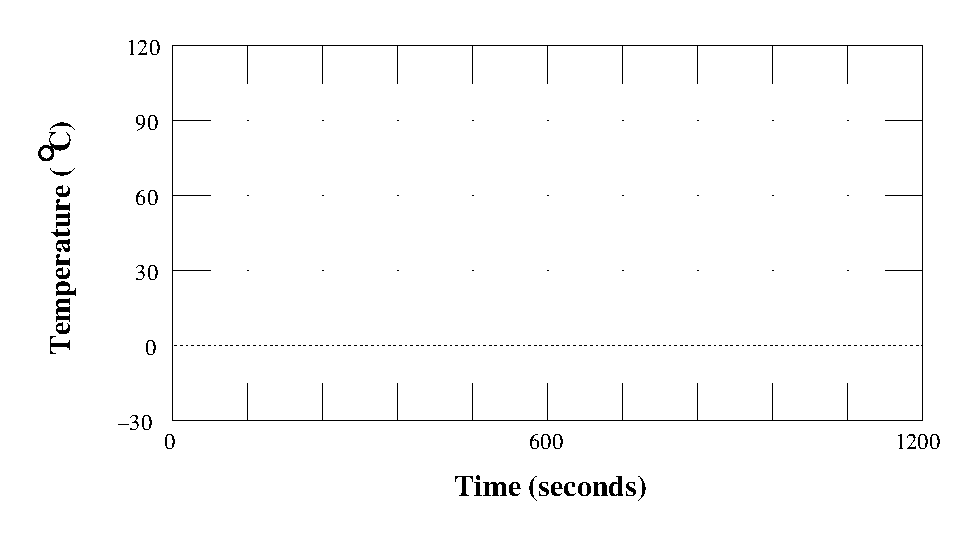
\includegraphics{heat_temp_int_energy_fig_1.eps} \par}
\vspace{0.3cm}

\textbf{Activity 2: Measuring T vs. t for Water} 

(a) To test your prediction: 

\begin{enumerate}
\item Fill the hypsometer (boiler) at least half full of ice water and suspend
the temperature probe so that the end is submerged in the ice water
but not touching the side or bottom of the hypsometer. 
\item Open the \textit{Heat, Temp, \& Internal Energy} application in the
132 Workshop folder on the {\bf Start} menu.
\item Light the burner and center it under the hypsometer. Click on the
\textbf{Start} button to begin recording data. The temperature of
the water will be recorded on the graph shown on the monitor. While
there is still ice, stir gently. 
\item After the water begins to boil, turn off the burner and stop collecting
data using the \textbf{Stop} button on the front panel. 
\item Sketch the shape of the measured heating curve on the above graph
using a solid line. Ignore small variations due to noise and uneven
heating. Mark the points at which the ice has melted and the water
begins to boil.
\end{enumerate}
(b) Does your prediction agree with the measured heating curve? If
not, what are the differences?
\vspace{20mm}

(c) What is the relationship between the temperature and the added
heat while the ice is melting?
\vspace{20mm}

(d) What is the relationship between the temperature and the added
heat after the ice has melted, but before the water begins to boil?
\vspace{20mm}

(e) What is the relationship between the temperature and the added
heat while the water is boiling?
\vspace{20mm}

(f) If there are regions of the heating curve in which the temperature
is not changing, what do you think is happening to the added heat
in these regions?\vspace{20mm}

